%\IEEEraisesectionheading{\section{Introduction}\label{sec:introduction}}
\section{Introduction}
% Computer Society journal (but not conference!) papers do something unusual
% with the very first section heading (almost always called "Introduction").
% They place it ABOVE the main text! IEEEtran.cls does not automatically do
% this for you, but you can achieve this effect with the provided
% \IEEEraisesectionheading{} command. Note the need to keep any \label that
% is to refer to the section immediately after \section in the above as
% \IEEEraisesectionheading puts \section within a raised box.




% The very first letter is a 2 line initial drop letter followed
% by the rest of the first word in caps (small caps for compsoc).
% 
% form to use if the first word consists of a single letter:
% \IEEEPARstart{A}{demo} file is ....
% 
% form to use if you need the single drop letter followed by
% normal text (unknown if ever used by the IEEE):
% \IEEEPARstart{A}{}demo file is ....
% 
% Some journals put the first two words in caps:
% \IEEEPARstart{T}{his demo} file is ....
% 
% Here we have the typical use of a "T" for an initial drop letter
% and "HIS" in caps to complete the first word.
%\IEEEPARstart{T}{his} demo file is intended to serve as a ``starter file''
%for IEEE Computer Society journal papers produced under \LaTeX\ using
%IEEEtran.cls version 1.8b and later.
%% You must have at least 2 lines in the paragraph with the drop letter
%% (should never be an issue)
%I wish you the best of success.
%
%\hfill mds
%
%\hfill August 26, 2015

%\subsection{Subsection Heading Here}
%Subsection text here.

% needed in second column of first page if using \IEEEpubid
%\IEEEpubidadjcol

%\subsubsection{Subsubsection Heading Here}
%Subsubsection text here.


% An example of a floating figure using the graphicx package.
% Note that \label must occur AFTER (or within) \caption.
% For figures, \caption should occur after the \includegraphics.
% Note that IEEEtran v1.7 and later has special internal code that
% is designed to preserve the operation of \label within \caption
% even when the captionsoff option is in effect. However, because
% of issues like this, it may be the safest practice to put all your
% \label just after \caption rather than within \caption{}.
%
% Reminder: the "draftcls" or "draftclsnofoot", not "draft", class
% option should be used if it is desired that the figures are to be
% displayed while in draft mode.
%
%\begin{figure}[!t]
%\centering
%\includegraphics[width=2.5in]{myfigure}
% where an .eps filename suffix will be assumed under latex, 
% and a .pdf suffix will be assumed for pdflatex; or what has been declared
% via \DeclareGraphicsExtensions.
%\caption{Simulation results for the network.}
%\label{fig_sim}
%\end{figure}

% Note that the IEEE typically puts floats only at the top, even when this
% results in a large percentage of a column being occupied by floats.
% However, the Computer Society has been known to put floats at the bottom.


% An example of a double column floating figure using two subfigures.
% (The subfig.sty package must be loaded for this to work.)
% The subfigure \label commands are set within each subfloat command,
% and the \label for the overall figure must come after \caption.
% \hfil is used as a separator to get equal spacing.
% Watch out that the combined width of all the subfigures on a 
% line do not exceed the text width or a line break will occur.
%
%\begin{figure*}[!t]
%\centering
%\subfloat[Case I]{\includegraphics[width=2.5in]{box}%
%\label{fig_first_case}}
%\hfil
%\subfloat[Case II]{\includegraphics[width=2.5in]{box}%
%\label{fig_second_case}}
%\caption{Simulation results for the network.}
%\label{fig_sim}
%\end{figure*}
%
% Note that often IEEE papers with subfigures do not employ subfigure
% captions (using the optional argument to \subfloat[]), but instead will
% reference/describe all of them (a), (b), etc., within the main caption.
% Be aware that for subfig.sty to generate the (a), (b), etc., subfigure
% labels, the optional argument to \subfloat must be present. If a
% subcaption is not desired, just leave its contents blank,
% e.g., \subfloat[].


% An example of a floating table. Note that, for IEEE style tables, the
% \caption command should come BEFORE the table and, given that table
% captions serve much like titles, are usually capitalized except for words
% such as a, an, and, as, at, but, by, for, in, nor, of, on, or, the, to
% and up, which are usually not capitalized unless they are the first or
% last word of the caption. Table text will default to \footnotesize as
% the IEEE normally uses this smaller font for tables.
% The \label must come after \caption as always.
%
%\begin{table}[!t]
%% increase table row spacing, adjust to taste
%\renewcommand{\arraystretch}{1.3}
% if using array.sty, it might be a good idea to tweak the value of
% \extrarowheight as needed to properly center the text within the cells
%\caption{An Example of a Table}
%\label{table_example}
%\centering
%% Some packages, such as MDW tools, offer better commands for making tables
%% than the plain LaTeX2e tabular which is used here.
%\begin{tabular}{|c||c|}
%\hline
%One & Two\\
%\hline
%Three & Four\\
%\hline
%\end{tabular}
%\end{table}


% Note that the IEEE does not put floats in the very first column
% - or typically anywhere on the first page for that matter. Also,
% in-text middle ("here") positioning is typically not used, but it
% is allowed and encouraged for Computer Society conferences (but
% not Computer Society journals). Most IEEE journals/conferences use
% top floats exclusively. 
% Note that, LaTeX2e, unlike IEEE journals/conferences, places
% footnotes above bottom floats. This can be corrected via the
% \fnbelowfloat command of the stfloats package.


\subsection{The Popularity of Voice Authentication on Smartphones}

According to reports issued by several market-research firms, the total number of smartphone users worldwide is over 3 billion this year and is expected to reach 3.9 billion by 2023~\cite{report2018newzoo,report2019forrester}. The rapid increasing use of smartphones is actuating the need for better protection. User authentication on smartphones has thus been an important area of research. 

Survey papers~\cite{vongsingthong2014survey,mahfouz2017survey,shankar2018survey} have compared the strengths and limitations of existing authentication methods, from knowledge-based methods such as PIN or password, to identity-based methods such as fingerprint and face.
%
PIN or password are the most widely used authentication methods. However, when the users have wet or dirty fingers, or wear gloves on their hands, such touchscreen-related authentication methods will not work. The fingerprint authentication suffers from the same problem. As for face recognition, it stops working when users are wearing moisturizing mask sheets or other head wearables such as ski goggles. In the aforementioned scenarios, voice authentication provides better convenience to users and thus a great alternative.


In fact, voice authentication has been adopted in a wide variety of smartphone applications. 
For example, Android users can say ``Ok Google'' to access Google assistant directly~\cite{onlinegoogle}; the Tencent company adopts Voiceprint to provide securely, faster and easier log-ins to WeChat accounts, available on both Android and iOS platforms~\cite{onlinewechat}; the BioTrust uses voice biometrics to allow elderly and sick people to order prescription medication without the need to leave the house~\cite{onlinebio}; the Citi bank uses voice biometrics authentication system for phone banking, which reduces the number of tedious security questions~\cite{onlineciti}; the LMH Blockchain adopts Say-Tec~\cite{onlinesaytec} to authenticate, validate, process, and protect users' blockchain assets and cryptocurrency by voice~\cite{onlineblockchain}.
%
Based on a market research report published in 2019~\cite{onlinemarket}, the speech and voice recognition market is expected to grow from 
 \$7.5 billion as in 2018 to  \$21.5 billion by 2024. 
 
 

\subsection{Voice Spoofing Attacks}\label{sec:spoof}
Despite of the increasing trend for the adopting of voice authentication, this method is not unassailable, just like other methods. Researchers have found that voice authentication system are vulnerable to the following four attacks~\cite{wu2015spoofing}: impersonation attack, replay attack, speech synthesis, and voice conversion.
\begin{itemize}
	\item  Impersonation attack refers to the scenario where an attacker tries to mimic the legitimate user’s voice without any computer-aided technology.
	\item Replay attack refers to the scenario where an attacker replays a pre-recorded speech sample collected from the legitimate user. 
	\item Speech synthesis refers to the scenario where an attacker generates intelligible, natural-sounding artificial speech from text.
	\item Voice conversion refers to the scenario where an attacker converts his speech signals to an artificial speech signal which has similar timbre and prosody to that of the legitimate user.
\end{itemize}


Among the four voice spoofing attacks, the impersonation attack is the hardest to perform, as Lau et al.~\cite{lau2005testing} have found that successful impersonation attacks require professional impersonators or attackers whose natural voices already similar to the legitimate user's. Even with professional mimicry artists or linguists, the existing voice authentication system is hard to fool~\cite{mariethoz2005can}.


The other three types of attacks, however, are much easier to be conducted. Because attackers could get the victim's voice recordings. It is common to see people use voice assistants (Alexa, Bixby, Cortana, Google, Siri, etc.) in public and attackers can record the victim's voice on the site or remotely. Moreover, people nowadays not only post text or image to social media sites (Facebook, Twitter, LinkedIn, YouTube, etc.), but also upload videos containing their voices. Attackers can extract the victim's voice from those online videos and build the speech profile of each victim. With a properly built speech profile, attackers are able to use the victim's voice to say just about anything, using algorithms such as vector quantization~\cite{abe1990voice}, probabilistic transform~\cite{stylianou1998continuous}, or neural networks~\cite{desai2009voice}. Such voice generation techniques are well-established. As an evidence, celebrity voice changer websites or apps could generate natural sounding speeches as from Obama, Trump, Stephen Hawking, Bruce Wayne, and many more.




Some may argue that large training data is required to build the victim's speech profile. However, for the purpose of attacking, the attackers may only need to use small training data to generate the hotword or the activation phrase. There is no need to generate every possible sentence. This is because most voice authentication systems adopts a one-time authentication scheme to grant access, instead of a continuous authentication scheme~\cite{feng2017continuous}.

\begin{landscape}
	\begin{figure*}[h]
		\begin{minipage}[t]{0.33\textwidth}
			\fbox{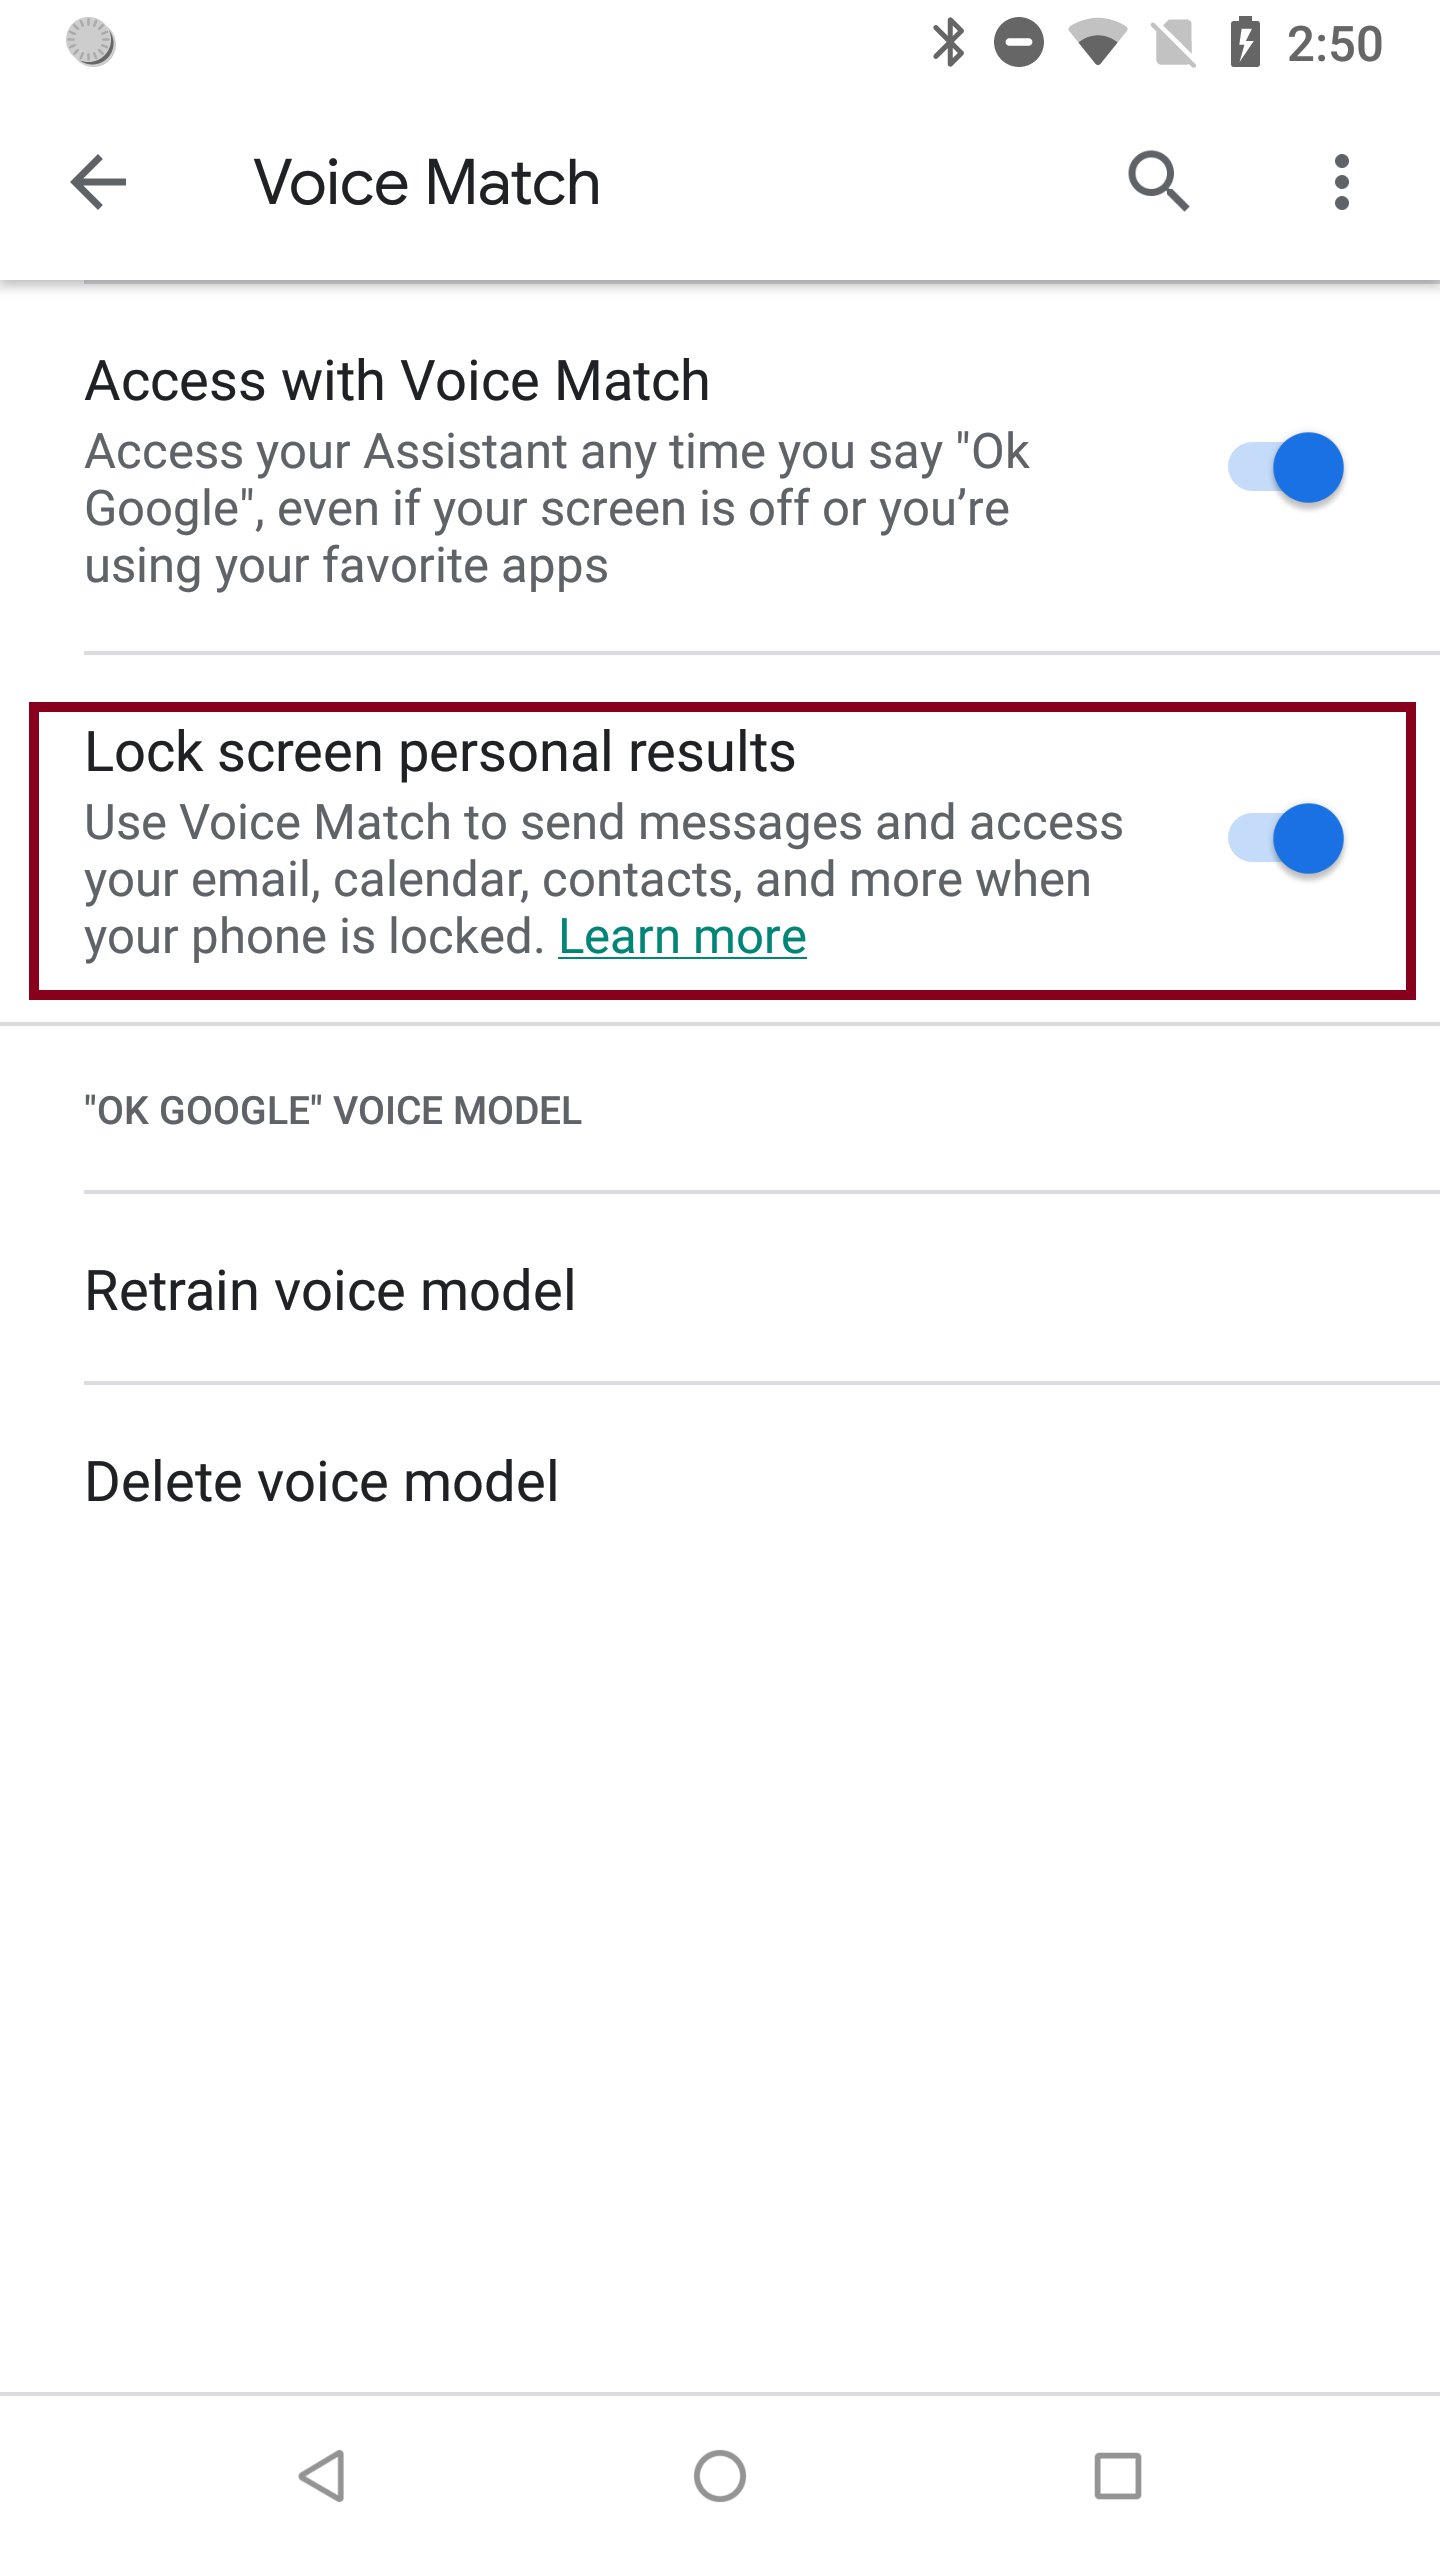
\includegraphics[width=1.2\textwidth]{voicematch}}
			\subcaption{Enabling Voice setting.}
			\label{fig:voicematch}
		\end{minipage}
		\hspace{1in}
		\begin{minipage}[t]{0.33\textwidth}
			\fbox{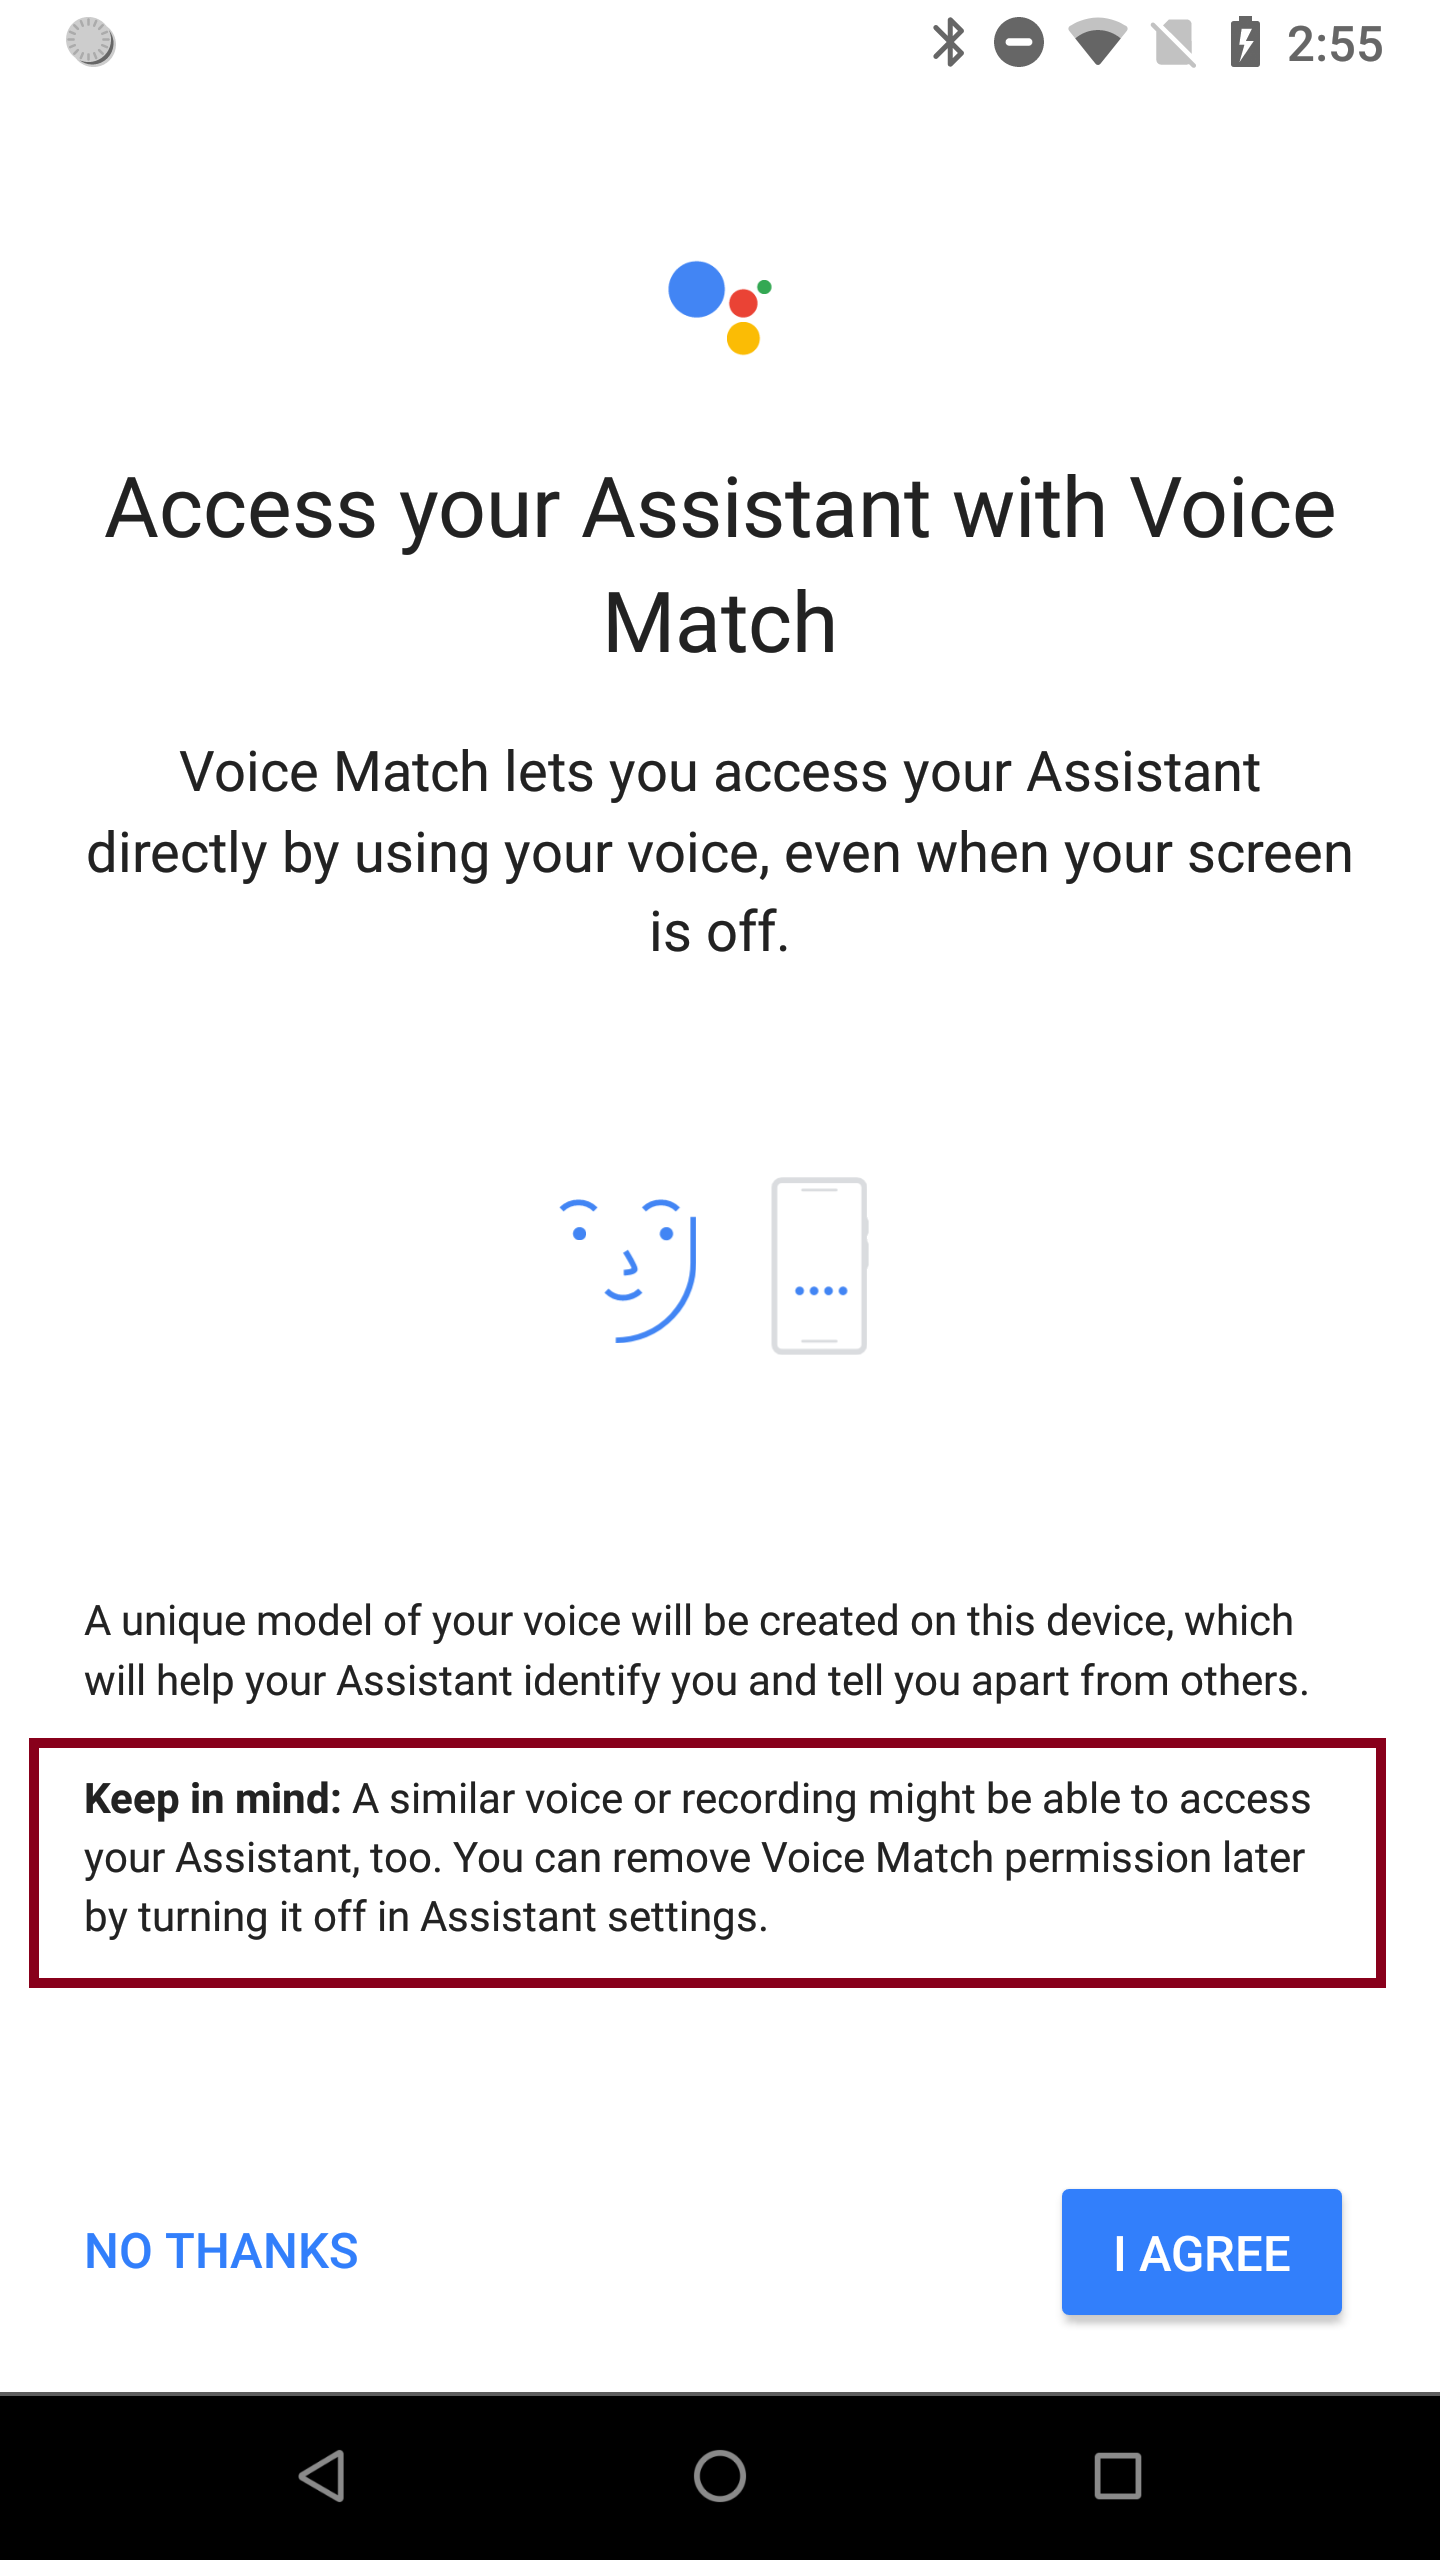
\includegraphics[width=1.2\textwidth]{voicematch2}}
			\subcaption{Voice Match warning.}
			\label{fig:voicematch2}
		\end{minipage}
		\hspace{1in}
		\begin{minipage}[t]{0.33\textwidth}
			\fbox{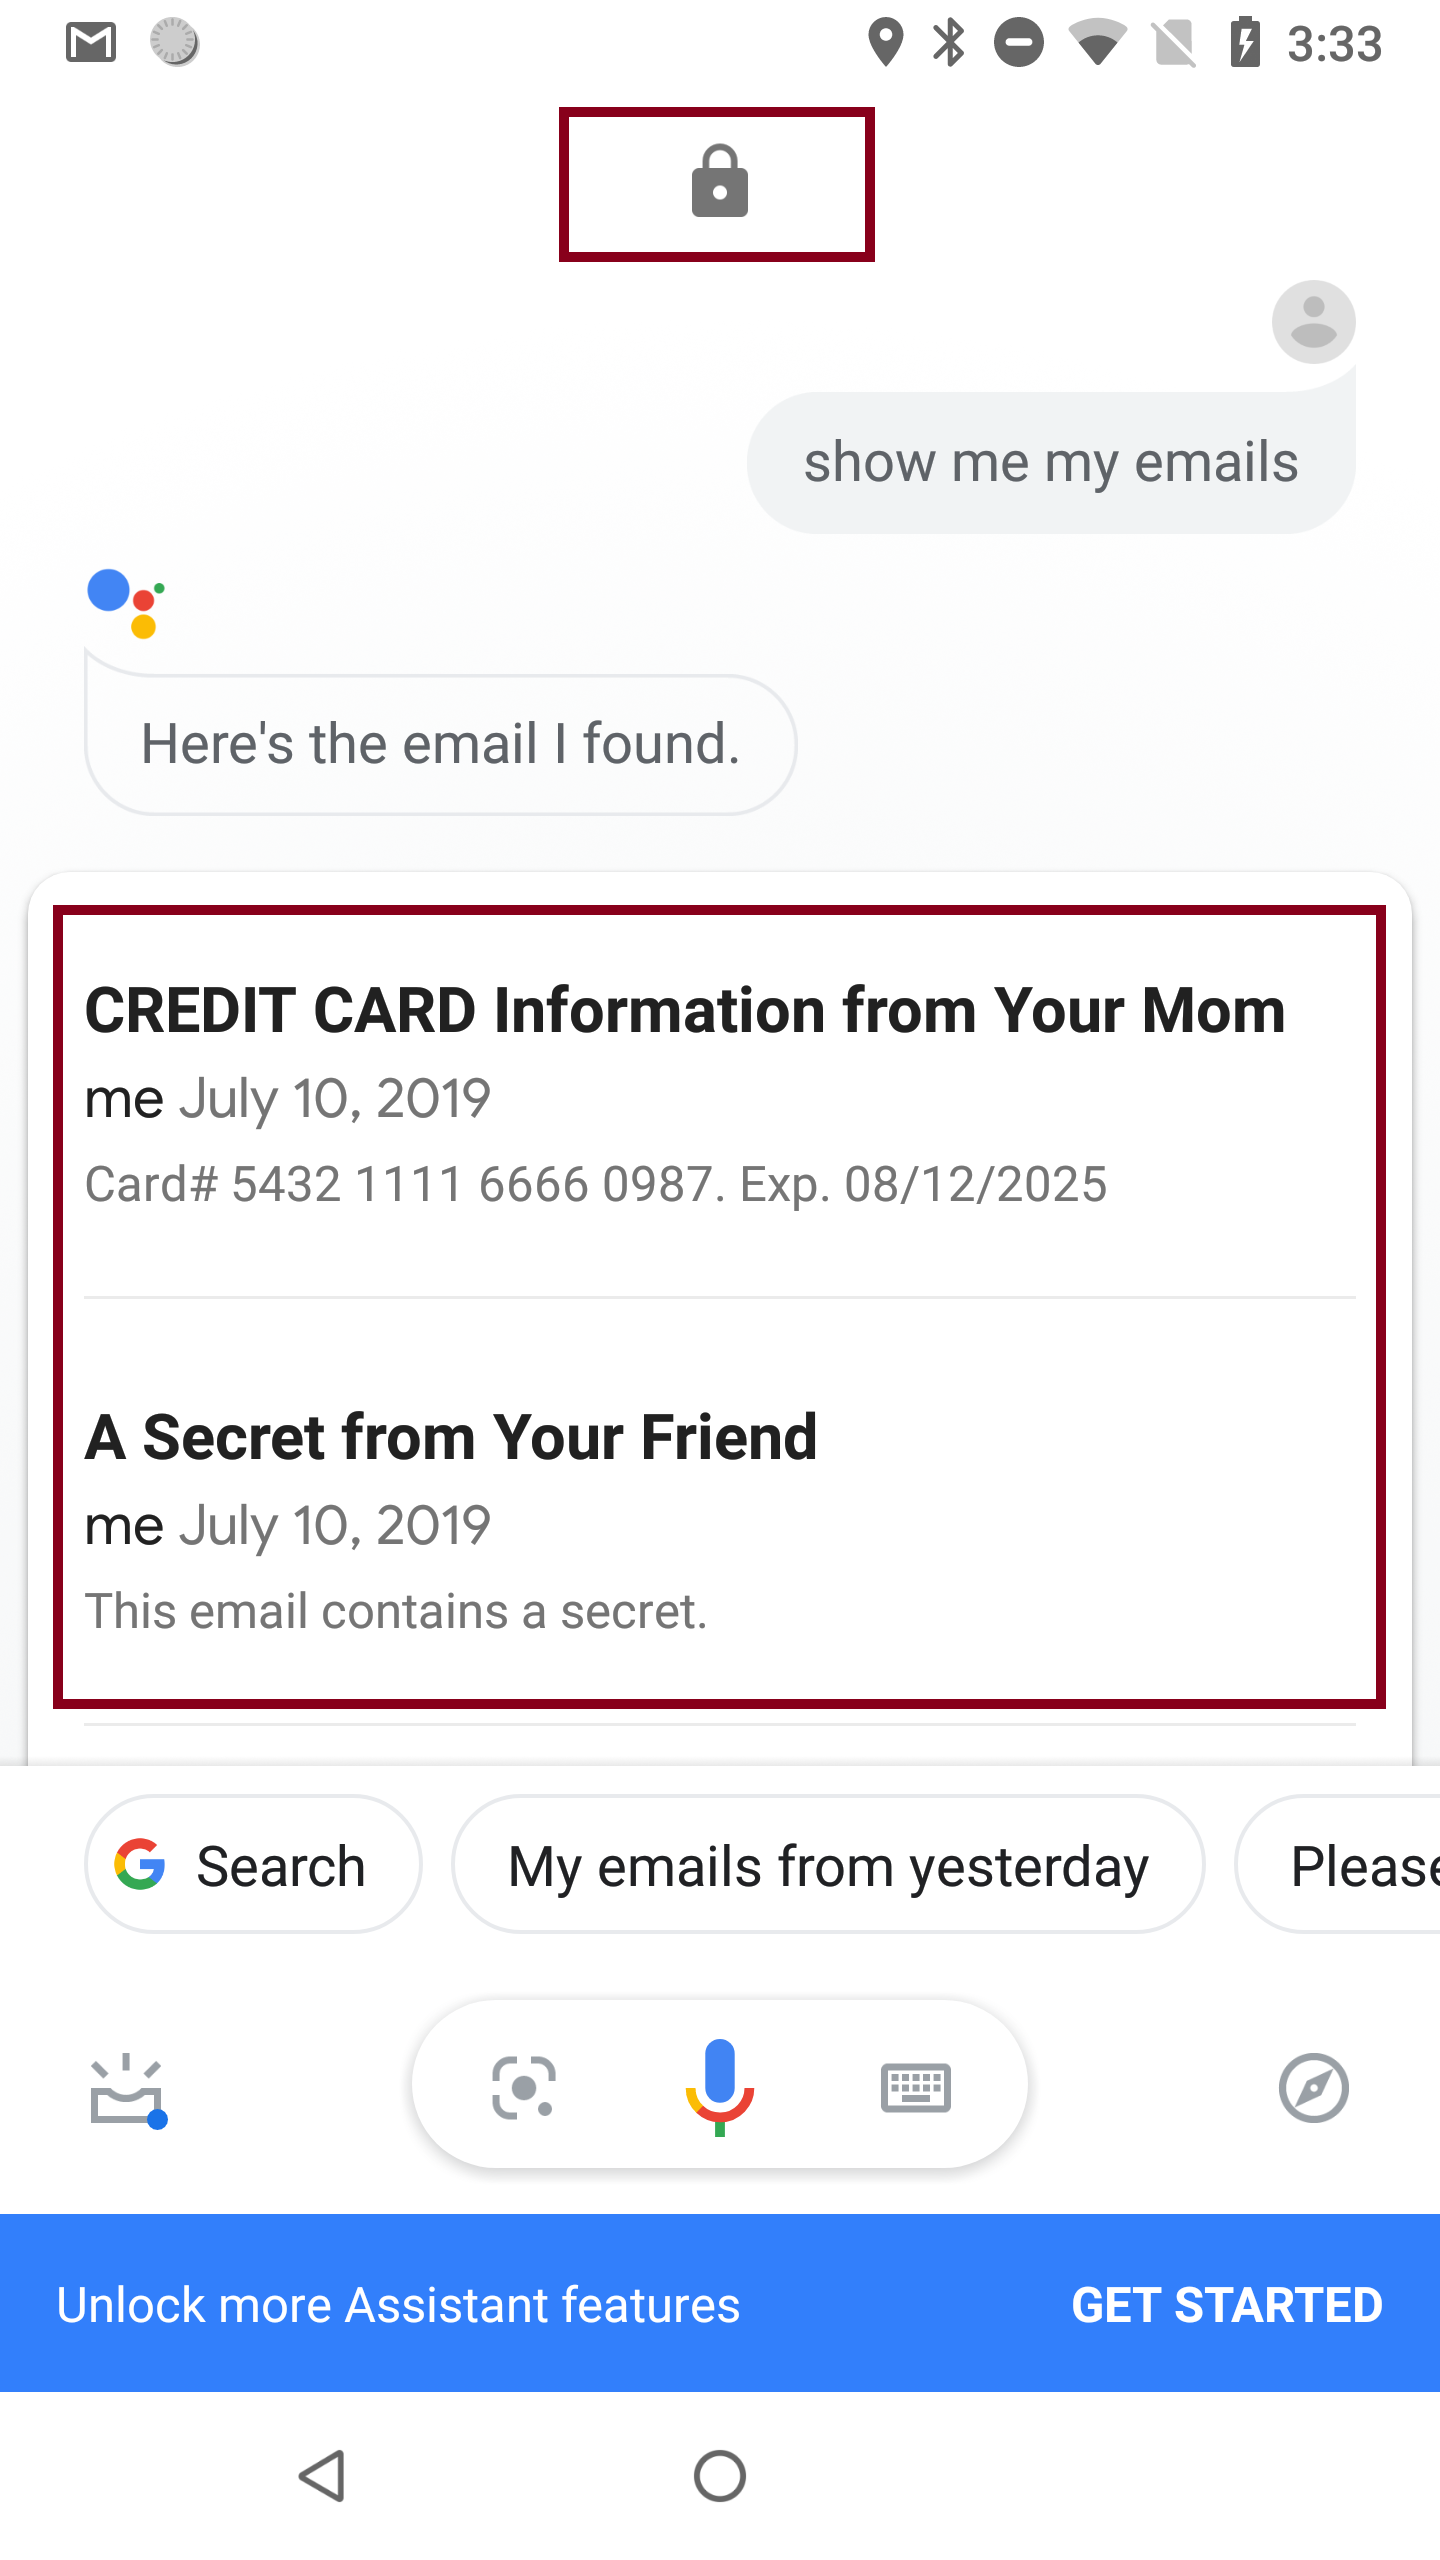
\includegraphics[width=1.2\textwidth]{email}}
			\subcaption{Information leakage when the phone is locked. }
			\label{fig:email}
		\end{minipage}  
	\vspace{-.05in}
		\caption{Screenshots about Voice Match on Google Nexus 6P.}\label{fig:example}
	\end{figure*}
\end{landscape}

For example, on a Google Nexus~6P smartphone running Android 8.1.0, it provides the Voice Match feature which allow users to access their personal data by voices\footnote{When the Voice Match feature first came out, Android users could fully unlock the phone with this function. However, starts from January 2019, Google removes the ability for Voice Match to act as a password due to security concerns. The previous ``Unlock with Voice Match'' is replaced to only providing ``personal results''. Such results come from emails, calendar entries, contacts, etc., and are still sensitive information.}. If an attacker replays the victim's ``Ok Google'' utterance, followed by ``show me my emails'' in his own voice (not the victim's), the Android system will regard him as the legitimate user (false acceptance) and show the emails. Because the authentication only check the hotword. Once the access is granted, any command coming after will be executed, no matter in whose voice.


Fig.~\ref{fig:example} are the screenshots when the aforementioned replay attack is tested in reality. Fig.~\ref{fig:voicematch} shows how to enable the Voice Match function. Fig.~\ref{fig:voicematch2} indicates the system is aware of its vulnerability to impersonation attack and replay attack. Fig.~\ref{fig:email} demonstrates the attacker could steal sensitive information without unlocking the phone (the closed padlock at the top). In this test, the leaked information are emails from the Gmail Inbox, which include the credit card information sent from the victim's mom and a secret from his friend. Recall that to conduct this attack successfully, all the thing the attacker need is a short recording of ``Ok Google'' in the victim's voice, but the harm can be huge.


\subsection{Liveness Detection}
Voice spoofing attacks drastically degrade the performance of standard voice authentication systems by increasing false acceptance rates~\cite{wang2011channel, ergunay2015vulnerability}, leading to severe security and privacy issues. Fortunately, researchers have done extensive research on defending these attacks and building spoof-proof voice authentication systems.




\begin{landscape}
	\SingleSpacing
	
	\begin{longtable}{p{3cm}p{6cm}p{6cm}ccc} %p{1.5cm}
		\caption{Related Work on Liveness Detection}
		\label{tab:liveness}
		\\
		
		\toprule
				Authors & Method & Shortcomming & Accuracy & \shortstack{No Extra \\ Devices} &  \shortstack{No Cumbersome \\ User Interaction}  \\
	%			& No User-specific Training\\
		\midrule
		
		\endfirsthead
		
		\normalfont\tablename~\thetable{}~Continued\\
		\toprule
				Authors & Method & Shortcomming & Accuracy & \shortstack{No Extra \\ Devices} &  \shortstack{No Cumbersome \\ User Interaction}  \\
	%			& No User-specific Training\\
		\midrule
		
		\endhead
		
		\bottomrule		
		\endfoot
		
		\endlastfoot
			Girija Chetty and Michael Wagner~\cite{chetty2004automated} & Detecting lip movements using cameras. & Inherits shortcomings of face authentication and introduces high computational overhead. & 99\% & \xmark & \cmark \\
%			& \xmark\\
			Poss et al.~\cite{poss2008biometric} & Using neural tree networks to determine unique aspects of utterances and Hidden Markov Models to classify them. & The accuracy is unkown. & - & \cmark & \cmark 
			\\
%			& \xmark \\
			Wei Shang and Maryhelen Stevenson~\cite{shang2010score} & Testing whether an incoming recording shares the same originating utterance as any of N stored recordings. & Performance is largely based on the pre-stored recordings. & 88.1\%/93.2\% & \cmark & \cmark 
			\\
%			& \xmark \\
			Jes{\'u}s Villalba and Eduardo Lleida~\cite{villalba2011detecting} & Detecting noises and spectrum changes caused by far-field microphone and loudspeakers. & Limits the replay attackers to use far-field microphones. & 91\%-100\% & \cmark & \cmark \\
%			& \cmark \\
			Wang et al.~\cite{wang2011channel} & Detecting channel pattern noise caused by microphone and loudspeakers. & Limits the replay attackers to use low-quality microphones. & 97\% & \cmark & \cmark 
			\\
%			& \cmark \\			
			Aley-Raz et al.~\cite{aley2013device}  & Integrating intra-session voice variation to Nuance VocalPassword~\cite{onlinenuance}. & Requires the user to cumbersomely repeat prompted sentences. & - & \cmark & \xmark 
			\\
%			& \cmark \\
			Zhang et al.~\cite{zhang2016voicelive} & \textbf{VoiceLive}: Measuring the time-difference-of-arrival changes of a sequence of phoneme sounds to the two microphones of the phone. & Requires at least two high-quality microphones in one smartphone. & 99\% & \cmark & \cmark 
			\\
%			& \xmark \\
			Chen et al.~\cite{chen2017you} & Detecting the magnetic field emitted from loudspeakers. & Requires the user to move the smartphone with the predefined trajectory around the sound source. & 100\% & \cmark & \xmark 
			\\
%			& \cmark \\			
			Zhang et al. ~\cite{zhang2017hearing} & \textbf{VoiceGesture}: Leverages Dopler shifts in signals caused by users' articulatory gestures when speaking. & Requires high quality microphones and needs a longer computation time. & 99\% & \cmark & \cmark
			\\
%			 & \xmark \\
			Feng et al.~\cite{feng2017continuous}  & \textbf{VAuth}: Utilizing the instantaneous consistency of the entire signal from the accelerometer and the microphone. & Requires the user to wear high-sampling-rate accelerometers on the facial, throat, or sternum areas. & 97\% & \xmark & \cmark 
			\\
%			& \cmark \\
			Huang et al.~\cite{huang2018breathlive}  & \textbf{BreathLive}: Utilizing chest movement when making deep breaths & The sound is deep breath sound instead of human speech; Stethoscope is needed. & 91\%/94\%/96\% & \xmark & \cmark 
			\\
%			& \xmark \\
			Ment et al.~\cite{meng2018wivo} & \textbf{WiVo}: Using channal state information (CSI) from WiFi signals to detect mouth movement  &  Requires WiFi antennas to collect the CSI info; the distance between antennas and human is short (20cm). & 99\% & \xmark & \cmark
 \\
\bottomrule

\end{longtable}

\end{landscape}

%\begin{landscape}	
%	\begin{table}
%		\centering
%%		\renewcommand{\arraystretch}{1.5}
%%		\caption{Related Work on Liveness Detection}
%%		\label{tab:liveness}
%		\footnotesize
%		\begin{tabular}{p{2.5cm}p{0.5cm}p{4.5cm}p{4.5cm}ccc} %p{1.5cm}
%			\toprule\specialrule{0.5pt}{1.5pt}{\belowrulesep}
%			Authors & Year & Method & Shortcomming & Accuracy & \shortstack{No Extra \\ Devices} &  \shortstack{No Cumbersome \\ User Interaction}  \\
%%			& No User-specific Training\\
%			\midrule
%			Girija Chetty and Michael Wagner~\cite{chetty2004automated} & 2004 & Detecting lip movements using cameras. & Inherits shortcomings of face authentication and introduces high computational overhead. & 99\% & \xmark & \cmark \\
%%			& \xmark\\
%			Poss et al.~\cite{poss2008biometric} & 2008 & Using neural tree networks to determine unique aspects of utterances and Hidden Markov Models to classify them. & The accuracy is unkown. & - & \cmark & \cmark 
%			\\
%%			& \xmark \\
%			Wei Shang and Maryhelen Stevenson~\cite{shang2010score} & 2010 & Testing whether an incoming recording shares the same originating utterance as any of N stored recordings. & Performance is largely based on the pre-stored recordings. & 88.1\%/93.2\% & \cmark & \cmark 
%			\\
%%			& \xmark \\
%			Jes{\'u}s Villalba and Eduardo Lleida~\cite{villalba2011detecting} & 2011 & Detecting noises and spectrum changes caused by far-field microphone and loudspeakers. & Limits the replay attackers to use far-field microphones. & 91\%-100\% & \cmark & \cmark \\
%%			& \cmark \\
%			Wang et al.~\cite{wang2011channel} & 2011 & Detecting channel pattern noise caused by microphone and loudspeakers. & Limits the replay attackers to use low-quality microphones. & 97\% & \cmark & \cmark 
%			\\
%%			& \cmark \\			
%			Aley-Raz et al.~\cite{aley2013device}  & 2013 & Integrating intra-session voice variation to Nuance VocalPassword~\cite{onlinenuance}. & Requires the user to cumbersomely repeat prompted sentences. & - & \cmark & \xmark 
%			\\
%%			& \cmark \\
%			Zhang et al.~\cite{zhang2016voicelive} & 2016 & \textbf{VoiceLive}: Measuring the time-difference-of-arrival changes of a sequence of phoneme sounds to the two microphones of the phone. & Requires at least two high-quality microphones in one smartphone. & 99\% & \cmark & \cmark 
%			\\
%%			& \xmark \\
%			Chen et al.~\cite{chen2017you} & 2017 & Detecting the magnetic field emitted from loudspeakers. & Requires the user to move the smartphone with the predefined trajectory around the sound source. & 100\% & \cmark & \xmark 
%			\\
%%			& \cmark \\			
%			Zhang et al.~\cite{zhang2017hearing} & 2017 & \textbf{VoiceGesture}: Leverages Dopler shifts in signals caused by users' articulatory gestures when speaking. & Requires high quality microphones and needs a longer computation time. & 99\% & \cmark & \cmark
%			\\
%%			 & \xmark \\
%			Feng et al.~\cite{feng2017continuous}  & 2017 & \textbf{VAuth}: Utilizing the instantaneous consistency of the entire signal from the accelerometer and the microphone. & Requires the user to wear high-sampling-rate accelerometers on the facial, throat, or sternum areas. & 97\% & \xmark & \cmark 
%			\\
%%			& \cmark \\
%			Huang et al.~\cite{huang2018breathlive}  & 2018 & \textbf{BreathLive}: Utilizing chest movement when making deep breaths & The sound is deep breath sound instead of human speech; Stethoscope is needed. & 91\%/94\%/96\% & \xmark & \cmark 
%			\\
%%			& \xmark \\
%			Ment et al.~\cite{meng2018wivo} & 2018 & \textbf{WiVo}: Using channal state information (CSI) from WiFi signals to detect mouth movement  &  Requires WiFi antennas to collect the CSI info; the distance between antennas and human is short (20cm). & 99\% & \xmark & \cmark
%			\\
%		\specialrule{0.5pt}{\aboverulesep}{1.5pt}\bottomrule
%		\end{tabular}
%	\end{table}
%\end{landscape}

%Shang et al.~\cite{shang2010score} propose to compare an input voice sample with stored instances of past accesses to detect the voice samples have been seen before by the authentication system. This method, however, cannot work if the attacker records the voice samples during a non-authentication time point. Villalba et al. and Wang et al. suggest that the additional channel noises introduced by the recording and loudspeaker can be used for attack detection~\cite{villalba2011detecting,wang2011channel}.
%These approaches however have limited effec- tiveness in practice. For example, the false acceptance rates of these approaches are as high as 17\%. Chetty and Wagner propose to use video camera to extract lip movements for liveness verification~\cite{chetty2004automated}, whereas Poss et al. combine the techniques of a neural tree network and Hidden Markov Models to improve authentication accuracy~\cite{poss2008biometric}.
%Aley-Raz et al.~\cite{aley2013device} develop a liveness detection system based on ``Intra-session voice variation'', which is integrated into Nuance VocalPassword~\cite{onlinenuance}. In addition to a user-chosen passphrase, it requires a user to repeat one or more random sentences prompted by the system for liveness detection. Such a method however increases the op- eration overhead of the user and is cumbersome due to an explicit user cooperation is required besides the standard authentication process. 
%
%More recently, Chen et al.~\cite{chen2017you} develop a smartphone based liveness detection system by measuring the magnetic field emit- ted from loudspeakers. It however requires the user to speak the passphrase while moving the smartphone with predefined trajectory around the sound source. Moreover, Zhang et al.~\cite{zhang2016voicelive} propose a smarthphone based solution, which measures the time-difference-of-arrival (TDoA) changes of a sequence of phoneme sounds to the two microphones of the phone when a user speaks a passphrase for liveness detection. However, it requires at least two high-accuracy microphones in one smartphone. Zhang et al.~\cite{zhang2017hearing} then propose VoiceGuesture, which leverages a user’s articulatory gestures when speaking a passphrase for liveness detection. However, the calculation overhead is high.
%Feng et al.~\cite{feng2017continuous} present VAuth,  which utilizes the instantaneous consistency of the entire signal from the accelerometer and the microphone.  However, it requires the user to wear a security-assisting device on the facial, throat, or sternum areas. 
%Huang et al.~\cite{huang2018breathlive} present BreathLive, which utilize the inherent correlation between sounds and chest motion caused by deep breathing to realize a reliable liveness detection system. However, it requires special gyroscope and stethoscope. Since it utilizes deep breathing, the sound period is very long (4 sec. for one deep breathing).
%
%In conclusion, the aforementioned approaches either require cumbersome user interaction, or require extra electronic devices, or require long recording time or processing time. Building a good liveness detection component is still an open problem.

As mentioned in Section~\ref{sec:spoof}, the threat of impersonation attack is much less than that of the other three attacks, so impersonation attack is not a research focus. For replay attack, speech synthesis, and voice conversion, researchers have noticed that they have one thing in common -- the attacking sound is played by an electronic speaker\footnote{In this and many other papers, attackers must play the attacking sound near the targeted smartphone. We do not consider the scenario where sound files are directly injected. Because if attackers can inject sounds to the system, the phone is already hacked. So there is no need to go through the voice authentication procedure anymore.} rather than spoken by a real person. Therefore, if the authentication system can distinguish whether the sound comes from a live person or an electronic device, it would be immune from those voice spoofing attacks.



Existing liveness detection methods can be classified into two groups: detecting human-related characteristics, or detecting device-related characteristics. 

As listed in Table~\ref{tab:liveness}, there have been many researches on detecting human-related characteristics.  
Girija Chetty and Michael Wagner~\cite{chetty2004automated} use cameras to detect lip movements to detect liveness. However, their work requires the camera access and inherits the shortcomings of face authentication systems. Similarly, Meng et al.~\cite{meng2018wivo} tries to detect mouth movement, but from channel state information from WiFi signals. Their approach requires antenna pairs and the antennas are placed very close to human (20cm), which is not practical in reality.
Poss et al.~\cite{poss2008biometric} use neural tree networks to determine unique aspects of utterances and hidden Markov models to classify those features. However, their work requires high computing power and long processing time. 
Wei Shang and Maryhelen Stevenson~\cite{shang2010score} detect liveness by testing whether an incoming recording shares the same originating utterance as any of previously-stored recordings. However, the performance of their work is largely based on the previously-stored recordings. 
Aley-Raz et al.~\cite{aley2013device} integrate intra-session voice variation to Nuance VocalPassword~\cite{onlinenuance} for liveness detection, but they require the user to cumbersomely repeat prompted sentences.
Zhang et al.~\cite{zhang2016voicelive} detect liveness by measuring the time-difference-of-arrival changes of a sequence of phoneme sounds using the two microphones of the phone, which requires at least two high-quality microphones in one smartphone. They also propose another work~\cite{zhang2017hearing} to detect users' articulatory gestures when speaking. However, their work requires high quality microphones again and needs a longer computation time.
Last but not least, Feng et al.~\cite{feng2017continuous}  utilizes the instantaneous consistency of the entire signal from the accelerometer and the microphone for liveness detection. Their work is the most closely related work to ours. However,  their work requires the user to wear extra accelerometers on the facial, throat, or sternum areas. Moreover, the accelerometer used in their work requires a very high sampling rate (11,000 Hz), which cannot be supported by current smartphones. In this work, we are only using a 400 Hz sampling rate for the accelerometer and the gyroscope.

The aforementioned researchers detects the liveness of a user directly, but we can also detect the liveness from the reverse side: detecting the presence of electronic devices. For example, Jes{\'u}s Villalba and Eduardo Lleida~\cite{villalba2011detecting}  detect noises and spectrum changes caused by far-field microphone and loudspeakers. Wang et al.~\cite{wang2011channel} detect channel pattern noise caused by microphone and loudspeakers to identify replay attackers. However, they can only deal with attackers who use low-quality microphones to record the legitimate user's voices or record the voice at a long distance. More recently, Chen et al.~\cite{chen2017you} detects the magnetic field emitted from loudspeakers to identify attacks, but their work requires the user to move the smartphone with the predefined trajectory around the sound source.


In conclusion, liveness detection methods either detect the presence of human beings or the presence of electronic devices. Existing work has at least one of the following shortcomings: 1) requiring special or extra devices; 2) requiring cumbersome user interaction; 3) requiring high computing power or long processing time; 4) limited ability in defending against spoofing attacks. Therefore, building a spoof-proof voice authentication system is still an open problem.



%TODO computation power
%less energy
%sensitive to surrounding noise



\begin{figure}[!h]
	\centering
	\begin{subfigure}[t]{0.15\textwidth}
		\centering
		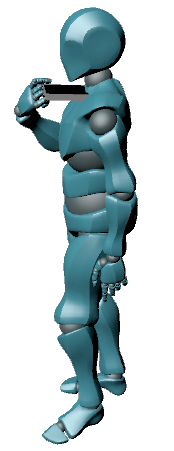
\includegraphics[height=1.8in]{standing}
		\caption{Standing}
	\end{subfigure}%
	~ 
	\begin{subfigure}[t]{0.15\textwidth}
		\centering
		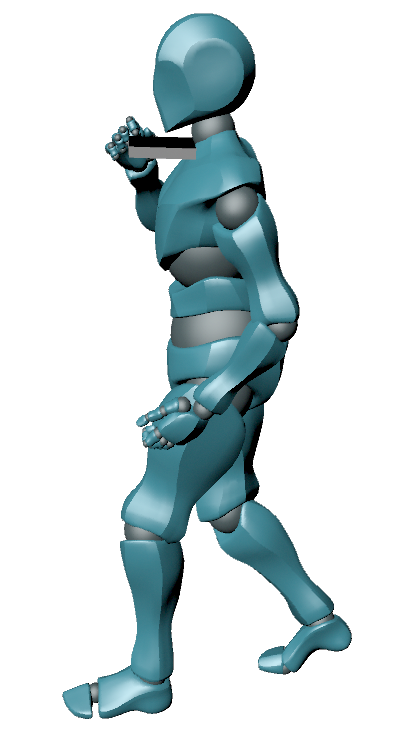
\includegraphics[height=1.8in]{walking}
		\caption{Walking}
	\end{subfigure}
	~ 
	\begin{subfigure}[t]{0.15\textwidth}
		\centering
		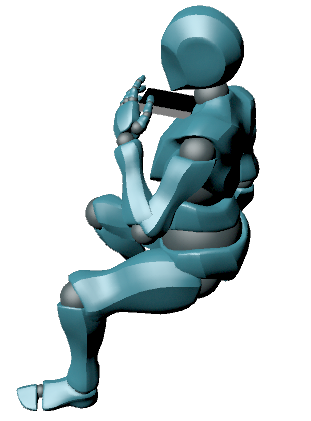
\includegraphics[height=1.8in]{sitting}
		\caption{Sitting}
	\end{subfigure}
	\caption{Authentication scenario of {\shortname}: holding the smartphone in contact with the throat while authenticating. In this way, the smartphone captures the body-borne voice vibrations through accelerometers and gyroscopes.}
	\label{fig:use}
\end{figure}

%TODO Add position test

\subsection{Overview of {\shortname}}

In this thesis, we propose {\shortname}, a spoof-proof voice authentication system that using \underline{mo}tion sensors (accelerometers and gyroscopes) to measure \underline{vo}ice.


As shown in Fig.~\ref{fig:use}, the user places the smartphone horizontally and makes sure the phone is in close contact with his throat. Then the embedded motion sensors inside the phone captures the conductive vibrations from vocal organs to the throat, and to the smartphone. Afterwards, the collected motion sensor data will be used for user authentication.


The intuition behind {\shortname} is the fact that human voice is essentially vibrations, so it can be recorded by motion sensors ~\cite{hopkin2003getting,o2009sonic,michalevsky2014gyrophone}.  Such motion-sensor data can be regarded as downsampled microphone data, so it has potentials to be used for voice authentication too. 
%
Moreover, since human body is a nonlinear medium similar to water~\cite{kim2014sound}, sounds go through the body will be affected by acoustic attenuation~\cite{szabo1994time} and self demodulation~\cite{berktay1965possible}. Such effects are human-only effects in that electronic devices are not water-like medium and have totally different acoustic properties. Therefore, using motion data for authentication can effectively differentiate live people from electronic devices, so that the system is protected against various voice spoofing attacks.

In fact,  there have been some recent studies that show the possibility of acquiring acoustic signals by smartphones' motion sensors. Michalevsky et al.~\cite{michalevsky2014gyrophone} proposed \textit{Gyrophone} in 2014. To the best of our knowledge, they are the first to use smartphone gyroscopes as low-frequency microphones to listen to loudspeakers. Gyrophone can differentiate 11 digits\footnote{One, two, \ldots, nine and zero.} with 65\% accuracy based on a 10 people dataset.
%
One year later, Zhang et al.~\cite{zhang2015accelword} proposed \textit{AccelWord}, which utilizes accelerometers to classify hotwords such as ``Okay Google'' or ``Hi Galaxy'' over other short phrases with 85\% accuracy. AccelWord is also tested over 10 people.
%
In 2018, however, Anald and Saxena~\cite{anand2018speechless} reproduced the aforementioned works and overturned their conclusions. They argued that smartphone motion sensors can not be affected by the speech signals transmitted through the air, no matter the sound source is a loudspeaker or a live person. They reported that only when the speakers and the motion sensors sharing a surface,  the  conductive vibrations will affect motion sensors' readings. Consisting with this newest research, {\shortname} asks the user to press the phone on his throat so that the body-borne vibrations are recorded, not the air-borne sounds.

%Except for this ``Loudspeaker-Same-Surface'' scenario, they studied 5 other  scenarios\footnote{``Loudspeaker-Different-Surface'',
%	``Laptop-Same-Surface'', `` Phone-Different-Surface'', 		``Human-Normal'',
%	and ``Human-Loud''.} and concluded that smartphone motion sensors only pose a limited threat to speech privacy.
% since conductive vibrations are ``possibly less common''.
%the impact of speech signals is very limited on motion sensors. 

%However, they missed one important scenario,  the \textit{intra-device} scenario, where the speakers and motion sensors are inside the same smartphone. The side-channel attack in this scenario, or the \textit{{\attackName}} attack as we refer to it, is the focus of this paper. We agree with Anald and Saxena on that motion sensors are more sensitive to conductive vibrations than aerial vibrations, but we show motion sensors can leak various critical information and pose a big threat to smartphone users' security and privacy. 


In summary, compared to previous works, the {\shortname} system have the following features:
\begin{itemize}
	\item  \textbf{All-in-One}: {\shortname} is an integral method which handles user authentication and liveness detection at the same time.
	
	\item  \textbf{Applicable}: {\shortname} works with current-off-the-shelf commercial smartphones. It does not require any extra electronic device nor any special phone model, since the sensors being used (motion sensors) are embedded on almost every smartphones.
	
	\item \textbf{Easy}: Except for pressing the smartphone on the user’s throat, {\shortname} does not ask users to do extra movements other than an ordinary speaking behavior.  
	
	\item \textbf{Improved Robust}: General voice authentication systems are sensitive to the surrounding noises and their performance will degrade a lot in noisy environments. {\shortname}, however, will not be affected. This is because smartphone's motion sensors measure the conductive vibrations and the  affection from air-borne sounds is very limited~\cite{anand2018speechless}.

%TODO change algorithms
%	\item \textbf{Computational Efficient}: {\shortname} has low computational overhead. For the same speech, motion data has a much smaller size  than that of microphones, because of the lower sampling rate (as shown in Table~\ref{tab:sample}). 
%%	Therefore, processing motion data is faster.
%	
%	\item \textbf{Energy Saving}: Motion sensors consume less energy than microphones ~\cite{zhang2015accelword}. 
	
	%TODO  section name
	\item \textbf{Expandable}: MoVo currently is a  text-dependent voice authentication systems that detects certain hotwords. However, it can be expanded to a text-independent system since it is syllable-based (will be elaborated in Section~\ref{sec:system}).
	
	
	%TODO accuracy	
%	\item
\end{itemize}




% and are dependent on the unique body structures of different people. Therefore, the data collected by motion sensors can be used for authentication and is spoof-proof.

%using the motion sensor measured voice to do authentication, instead of the microphone data, can effectively protect the system from voice spoofing attacks.



%
%As shown in Fig.~\ref{fig:use}, \shortname~records the user's voices by built-in microphones and the user's throat movement by the motion sensors at the same time. Only when these two types of signals match each other, the user is considered as a live person; otherwise, the user is rejected immediately.
%
%%\begin{figure}[!h]
%%	\centering
%%	\begin{tikzpicture}
%%	\draw (0, 1) node[inner sep=0] {\includegraphics[width=.2\linewidth]{use}};
%%	\draw (3, 1.5) node {\footnotesize\textsf{\qquad Speech -> Microphones} };
%%	\draw (4, 0) node {\footnotesize\textsf{\qquad throat Movement -> Accelerometers and Gyroscopes} };
%%	\end{tikzpicture}
%%	\caption{Authentication scenario of \shortname: placing the smartphone on the throat when speaking. In this way, the smartphone captures the audio signals by microphones and throat movements by motion sensors simultaneously.}
%%	\label{fig:use}
%%\end{figure}
%
%Although it is easy to be accepted that a person's voice and his throat movement are closely correlated,  the corresponding speech signals and motion data are not easy to be matched. The challenges are:
%\begin{itemize}
%	\item The gap between the sampling frequencies of different sensors is large. The microphone sensor on commercial off-the-shelf smartphones has a typically 44.1 kHz or 48 kHz sampling frequency~\cite{onlinemicrophone}, while the accelerometer and gyroscope has a typical 200 Hz maximum sampling frequency~\cite{michalevsky2014gyrophone}. Note that the inherent sampling frequency of MEMES sensors on smartphones is actually higher than the above values~\cite{suprem2017orientation}. However, the operating system restricts the rate.
%	\item The on-body vibration created by the sound production is subtle. Moreover, since the motion sensors are embedded in smartphones, they are not directly contacted, which further lowers the readings.
%	\item The noises caused by other body movements, heart beats, and breathings are strong interference. 
%\end{itemize}
%
%%TODO proof-of-concept
%
%%TODO figures about challenges
%\begin{figure}[h]
%%	\centering
%%	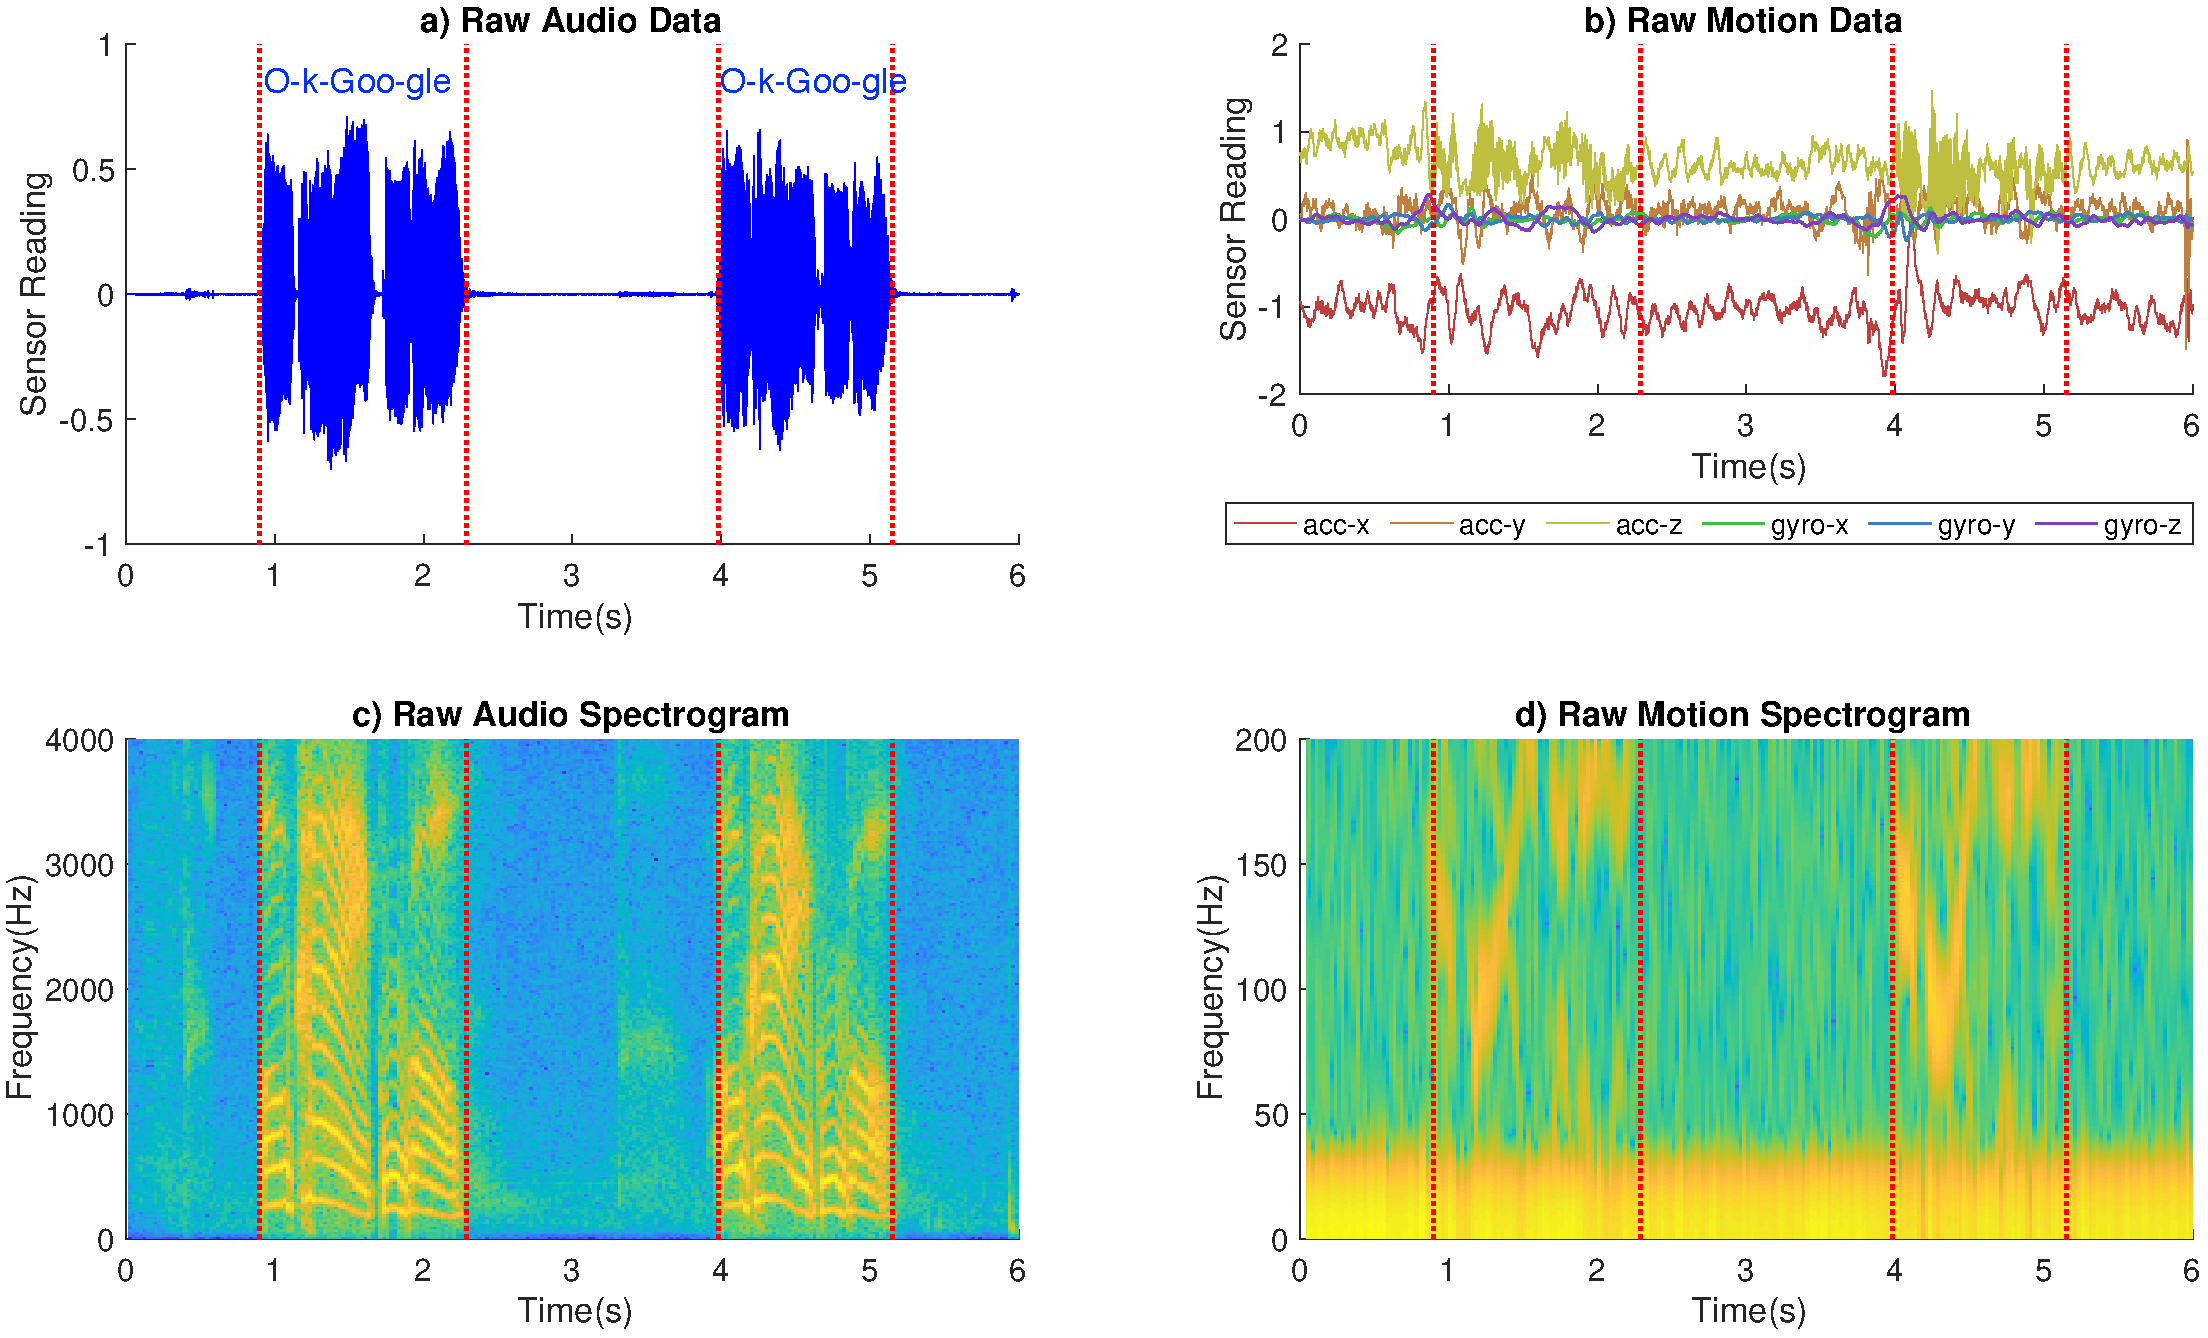
\includegraphics[height=.4\textheight]{SPSC}
%%	\caption{One user speaks ``Ok Google'' twice.}
%%	\label{fig:SPSC}
%%\end{figure}
%%%TODO more descriptions about the figure.
%%\begin{figure}[h]
%%	\centering
%%	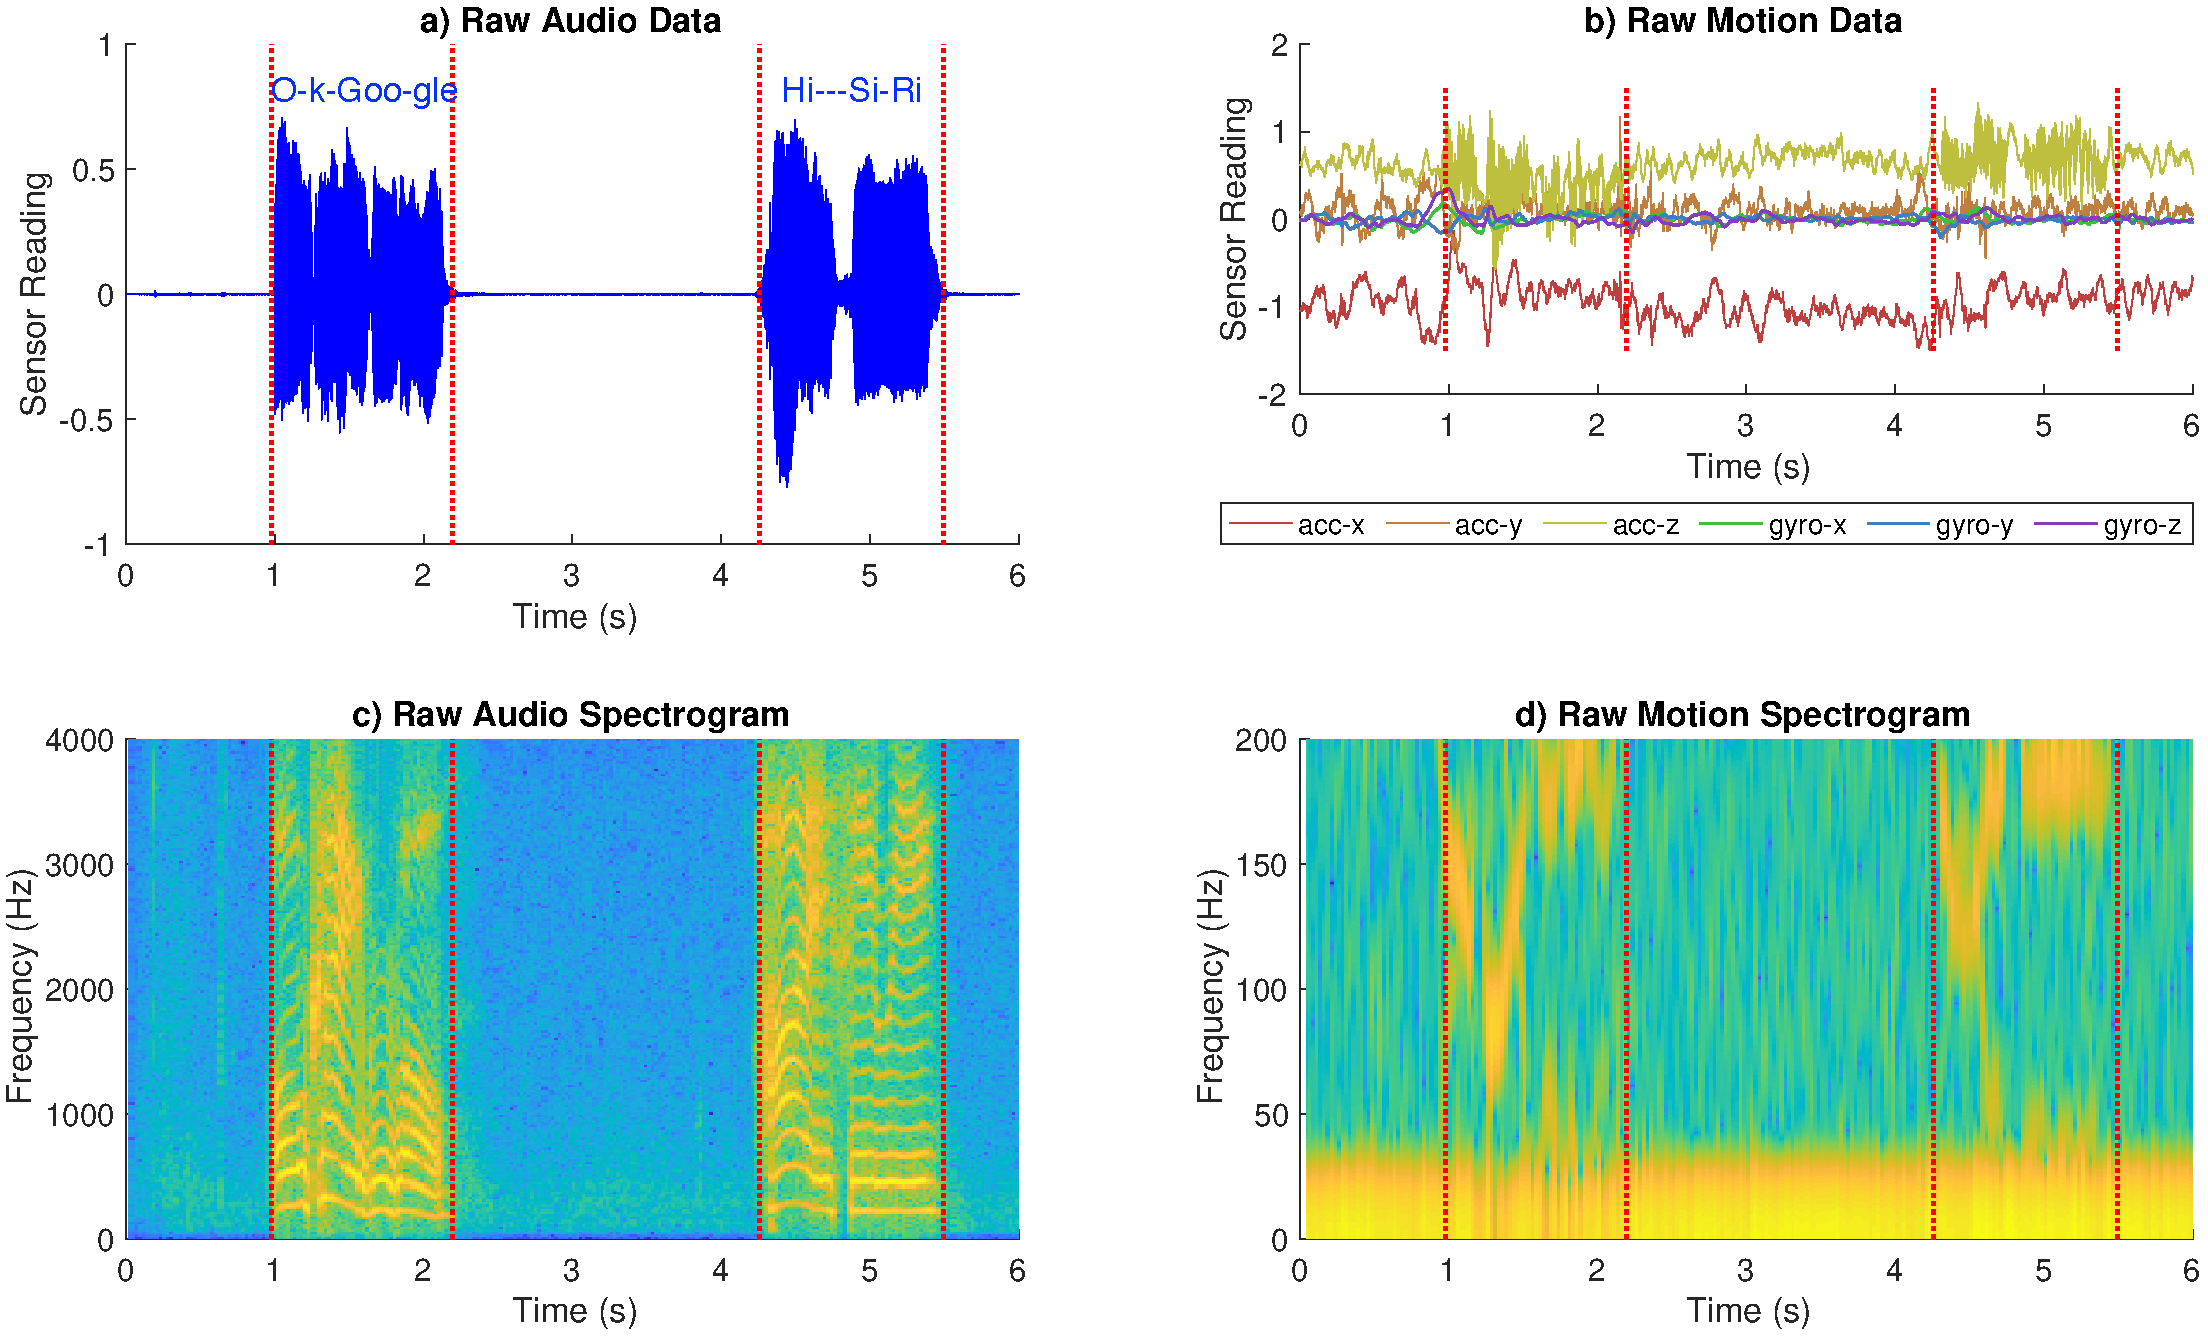
\includegraphics[height=.4\textheight]{SPDC}
%%	\caption{One user speaks ``Ok Google'' and ``Hi Siri''.}
%%	\label{fig:SPDC}
%%\end{figure}
%%\begin{figure}[h]
%%	\centering
%%	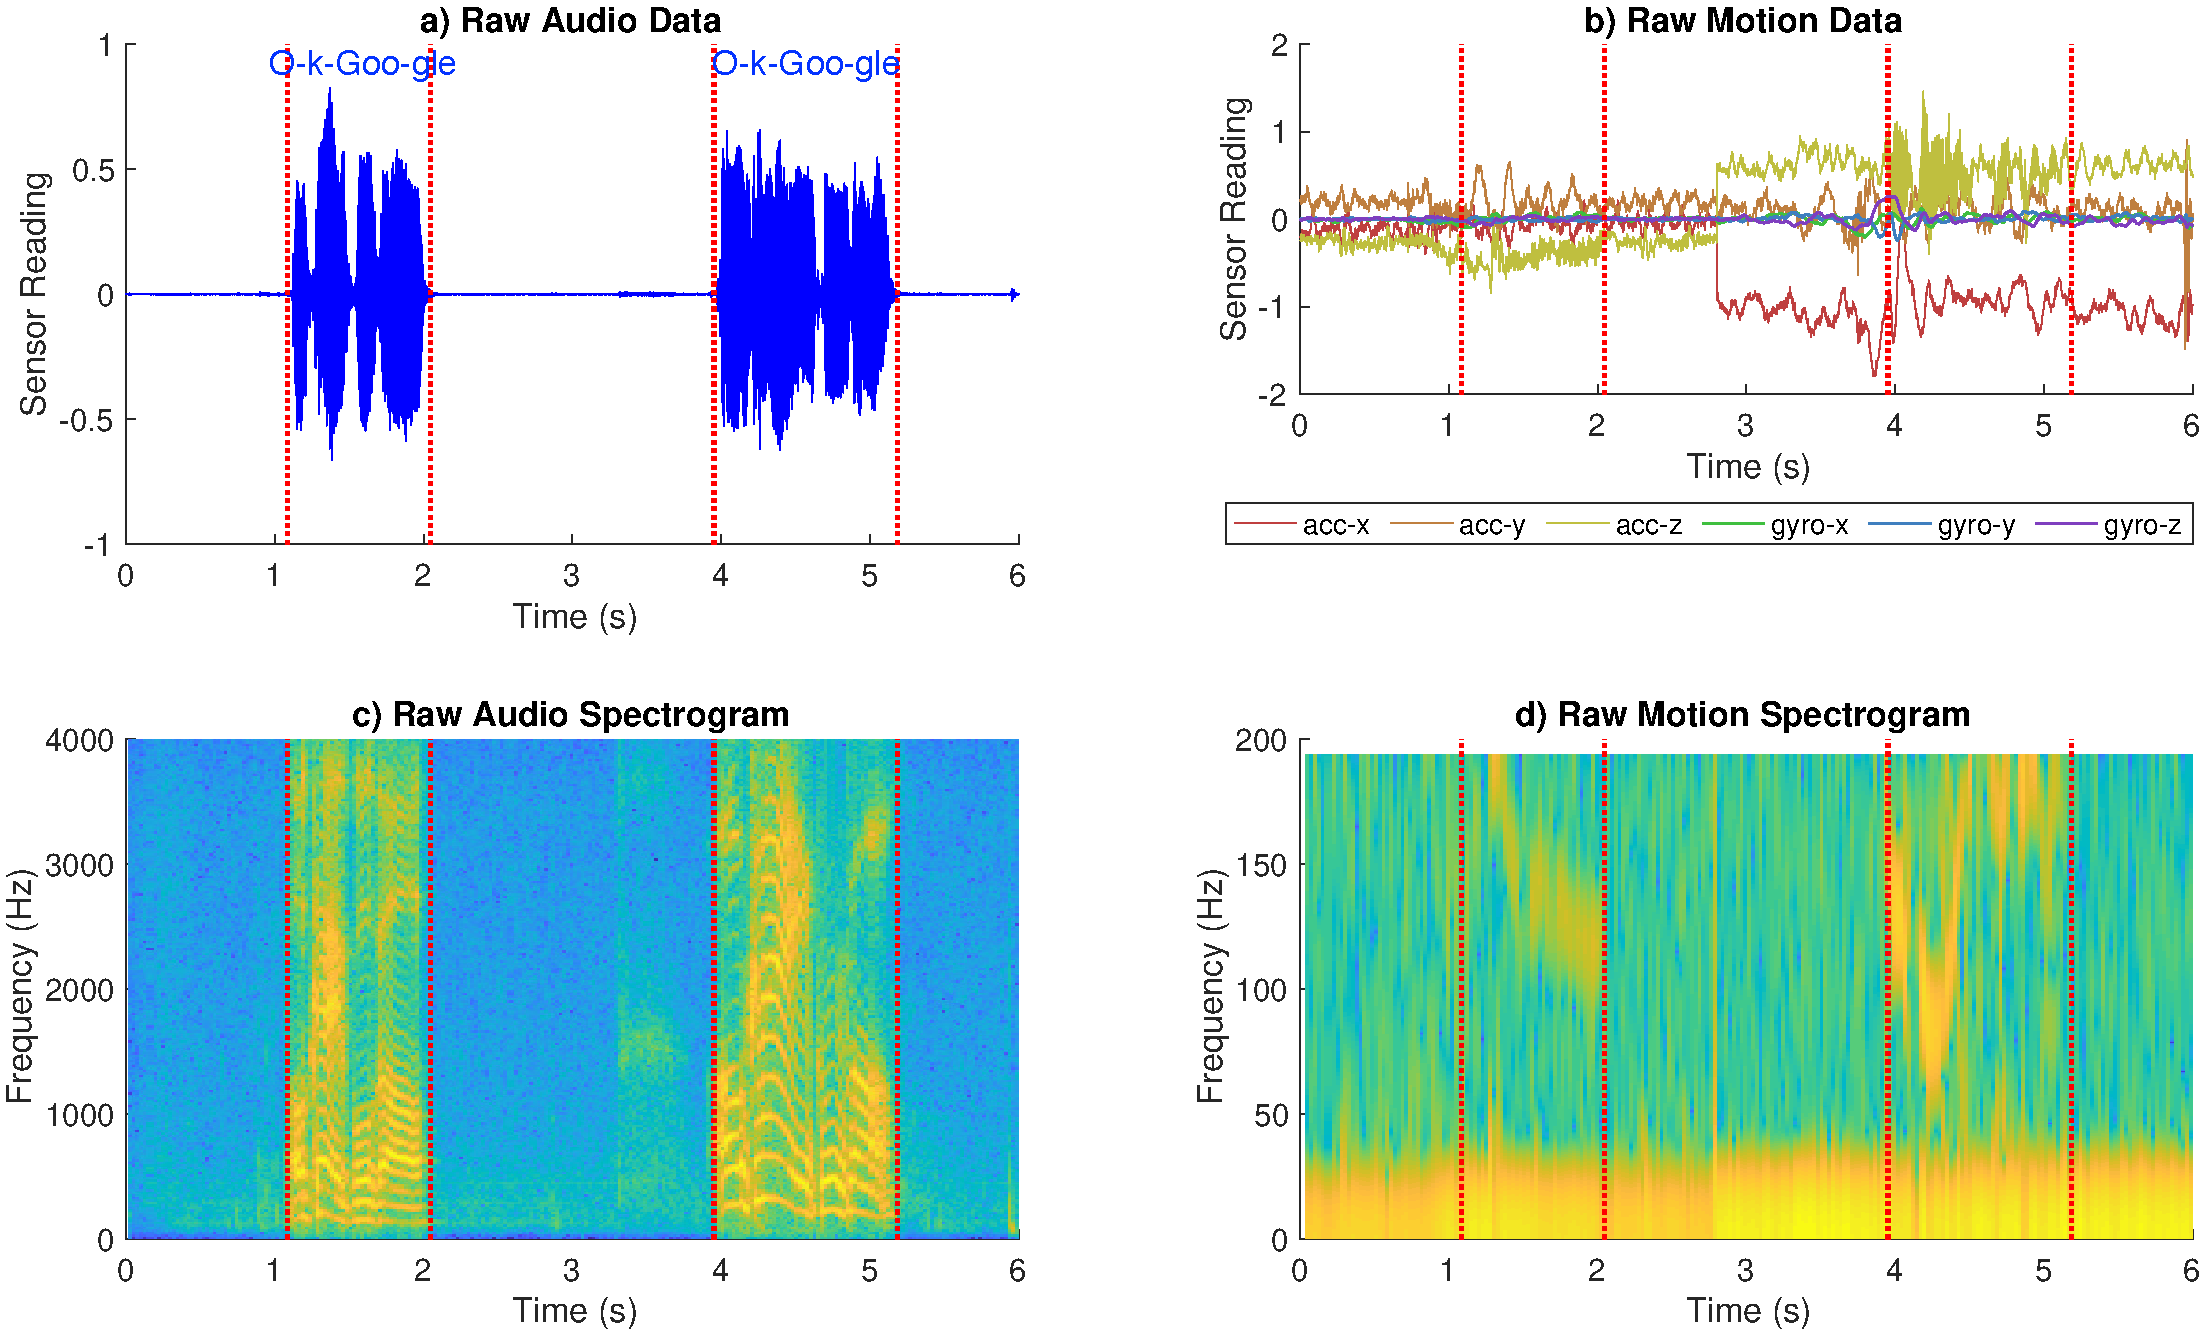
\includegraphics[height=.4\textheight]{DPSC}
%%	\caption{Different users both speak ``Ok Google''.}
%%	\label{fig:DPDC}
%%\end{figure}
%
%%TODO change same commands, do not fear DUPLICATION, ADDING HOW THE DATA IS COLLECTED
%%todo NO ()
%
%%TODO change plotted, are plotted, plot
%%WHY CHOOSE AXIS-Z
%\textbf{Proof-of-Concept}.
%Fig.~\ref{fig:SPSC}, Fig.~\ref{fig:SPDC}, and Fig.~\ref{fig:DPDC} show the example data when the same user speaks the same command ``Ok google'', the same user speaks different commands ``Ok google'' and ``Hi Siri'', and different users speak the same command ``Ok Google''. The data are collected as in Fig~\ref{fig:use}. The audio data is from the microphone with sampling rate 8,000 Hz while the motion data is sampled at 400Hz as it is the highest sample rate on Nexus 6P. In each figure, the left two subfigures, a) and c), are plotted based on microphone data, and the right two subfigures , b) and d),  are based on motion data; the top two subfigures, a) and b, plot time-domain data, while the bottom  two subfigures, c) and d), plot frequency-domain data. Note that the raw motion data have three dimensions, as shown in b) subfigures, but the spectrogram (d) subfigures only choose acc-z data to draw since it is the most representative one.
%%TODO
%
%%
%From these three figures, we can observe that the motion data are nosier and contain much fewer data and less representative than audio data, which are direct evidence of the aforementioned challenges. Note that in the ideal case, we expect when users speak the same command, no matter the same user or different users, the motion data should be similar. However, based on real data, as shown in Fig.~\ref{fig:DPDC} d), the raw spectrogram of different users are quite different. This is because different users have the different dominant speaking frequencies. What's worse, Fig.~\ref{fig:DPDC} d) shows the spectrograms are similar when one user speaks different commands.  Such observations indicate that frequency-domain data are not of much use to match between motion data and the same commands. Therefore, we adopt long short-term memory (LSTM) network, a variant of recurrent neural network (RNN), to learn the patterns of motion data in time-domain. 
%
%
%As elaborated in Section~\ref{sec:sys}, we also design syllable separation and majority voting components to further improve the performance of the LSTM network and increase the overall liveness detection accuracy.  In conclusion,  our \shortname~system has the following advantages:
%\begin{itemize}
%	\item \shortname~works with current-off-the-shelf commercial smartphones. It does not require any extra electronic device.
%	\item Except for pressing the smartphone on the user's throat, \shortname~does not ask users to do extra movements other than an ordinary speaking behavior. 
%	\item \shortname~can defend against at least 3*2= 6 different attacks. As elaborated in Section~\ref{sec:attack},  \shortname~protects the system against simple playback attack and sophisticated mimicry attack, where in each case, the speaker could play audio samples generated by replay attack, speech synthesis, or voice conversion. 
%	\item \shortname~does not require any user-specific training. Our matching algorithm is based on a user-independent model.
%	\item \shortname~currently works with text-dependent voice authentication systems. However, it is easy to expand the system to text-independent systems.
%\end{itemize}
